\section{Introduction}
\label{sec:introduction}

UAV-based cross-view geo-localization (UAV-CVGL) aims to infer the geographic location corresponding to a UAV-view observation by retrieving geo-referenced satellite images.~\cite{zheng2020university}.
This task can provide visual localization support for UAV autonomous navigation, emergency rescue and infrastructure inspection in GNSS-denied environments.
Due to differences in imaging viewpoint, observation scale and visible scene content, the same location can exhibit significantly different appearances across views, while different locations may share similar building layouts and surface textures.
To this end, existing studies typically learn location-discriminative and view-robust representations via global and local feature alignment~\cite{wang2022lpn,dai2022fsra,deuser2023sample4geo}.
However, practical deployment of UAV-CVGL requires mounting an offline-trained model on a UAV and applying it to unseen geographic regions under limited onboard computation and strict inference latency constraints.
Therefore, developing a lightweight and generalizable model that enables accurate UAV-satellite retrieval in unseen geographic regions is essential for translating UAV-CVGL research into practice.

\begin{figure}[t]
\centering
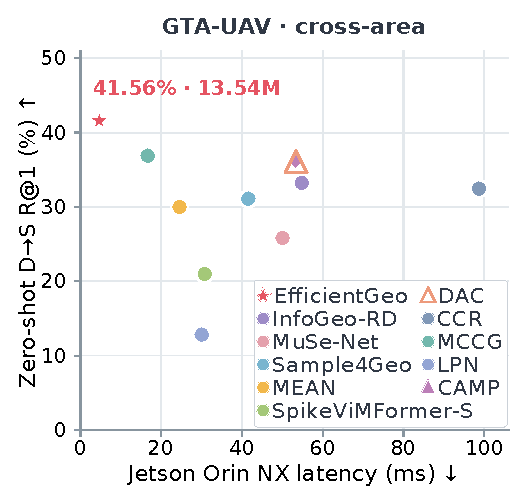
\includegraphics[width=\columnwidth]{EfficientGeo_GTA_CVPR_inside.pdf}


\caption{\textbf{Zero-shot retrieval accuracy versus query-encoding latency on Jetson Orin NX.} University-1652-trained models are evaluated on GTA-UAV cross-area.}
\label{fig:tradeoff}
\end{figure}

Motivated by this deployment requirement, some efforts have been made to pursue inference efficiency and reduce onboard cost through compact architectures, such as spike-driven transformer~\cite{chen2026spikevimformer} and ConvNeXt-Tiny backbones~\cite{chen2025mean}.
Another line of work targets cross-region generalization through object-centric structural alignment~\cite{zhang2026infogeo} and depth-aware geometric modeling~\cite{sun2026depthgeoloc}.
However, these two objectives are mutually constraining, since reducing model capacity may erode the representational richness that cross-region generalization depends on. This brings us to a fundamental question: how can we learn generalizable representations under strict model capacity constraints?

A promising direction is offered by self-supervised visual foundation models~\cite{caron2021dino,simeoni2025dinov3}, which encode general visual representations that transfer well across scenes and appearance variations. 
Such representations provide a strong prior for generalizable representation learning and help avoid overfitting to region-specific cues. 
However, task-agnostic foundation models are not aligned with the cross-view retrieval objective and even their compact variants can impose substantial computational demands for onboard inference.
Accordingly, this work focuses on transferring the generalization ability of a foundation model into a lightweight UAV-CVGL network for accurate UAV-satellite retrieval.

Knowledge distillation, which trains a compact student under the supervision of a stronger teacher, provides a natural route for such knowledge transfer~\cite{hinton2015distilling}. However, distilling a Transformer-based foundation model into a lightweight convolutional UAV-CVGL student is hindered by the substantial capacity gap and architectural discrepancy. 
Prior studies have shown that larger and stronger teachers do not guarantee better students~\cite{cho2019efficacy}, and that representation divergence across architectures further degrades feature-level distillation~\cite{liu2022crossarchitecture,hao2023ofa}.
Inspired by teacher assistant knowledge distillation~\cite{mirzadeh2020takd}, we insert a medium-scale, CVGL-specific Transformer as an intermediate teacher.
Architecturally homogeneous with the foundation teacher, it inherits the teacher's generalizable representations while specializing them for UAV-satellite retrieval. 
These intermediate descriptors are further turned into supervision targets tailored to the capacity and convolutional structure of the lightweight student, making the intermediate model a bridge between the foundation model and the compact student. 

In this paper, we propose EfficientGeo, a lightweight convolutional UAV-CVGL network trained through a two-stage distillation pipeline, in which a visual foundation model fine-tuned on the cross-view retrieval task serves as the teacher. 
In the first stage, we introduce Teacher-Guided Hard Negative Distillation (TG-HND), where the teacher identifies hard negatives and guides a Transformer-based intermediate model to mimic the corresponding positive-negative similarity margins.
Complementing this ranking guidance, multi-level feature calibration aligns the intermediate model’s hidden representations with fused features from multiple teacher layers, encouraging more discriminative feature learning.
In the second stage, Asymmetric Dual-Subspace Distillation (ADSD) projects the intermediate descriptor into a deterministic dominant subspace that carries its principal directions and an independently sampled random subspace that contributes complementary constraints, yielding low-dimensional supervision targets. Supervising these low-dimensional coordinates relieves the student from reproducing representational directions beyond its capacity, making cross-architecture supervision well-posed and helping to preserve the generalizable representations inherited in the first stage.

 Both stages further adopt distillation-guided Sharpness-Aware Minimization (SAM)~\cite{foret2021sam}  as an optimizer-level regularizer, which seeks flat minima for the distilled objectives and improves robustness. Through this pipeline, the lightweight EfficientGeo retains much of the generalization capability of the foundation model while remaining compact for onboard retrieval, achieving both efficient inference and generalizable cross-view geo-localization.

Our main contributions are summarized as follows:
\begin{itemize}
  \item We establish a two-stage cross-architecture distillation framework for UAV-CVGL that distill a fine-tuned visual foundation model to a lightweight convolutional student through a Transformer-based intermediate model, yielding EfficientGeo as a lightweight and generalizable solution for onboard cross-view geo-localization.
  \item We introduce ADSD for cross-architecture transfer. It projects each teacher descriptor onto principal directions and independently sampled random directions, then trains a separate student mapping for each fixed set of directions.
  \item Trained on University-1652, the reparameterized 13.54\,M-parameter student achieves zero-shot drone-to-satellite R@1 of 94.35\% on SUES-200, averaged over four flight heights, and 41.56\% on GTA-UAV cross-area. The same encoder encodes a query image in 4.65\,ms on Jetson Orin NX.

\end{itemize}

